\documentclass[10pt, conference]{IEEEtran}

%some packages we might use
\usepackage{subfigure}
\usepackage{graphicx}
\usepackage{graphicx, subfigure, epsfig, multirow}
% \usepackage[urlbordercolor={1 1 1}, linkbordercolor={1 1 1}]{hyperref}
\usepackage[urlbordercolor={1 1 1} ]{hyperref}
\usepackage[hyphenbreaks]{breakurl}
\usepackage{amssymb,amsmath}
% \usepackage[ruled,vlined]{algorithm2e}
\usepackage{algorithm}% http://ctan.org/pkg/algorithms
\usepackage{algpseudocode}% http://ctan.org/pkg/algorithmicx
\usepackage{color}
\usepackage{booktabs}

%this makes our life easy
\newcommand{\tabincell}[2]{\begin{tabular}{@{}#1@{}}#2\end{tabular}}
\newcommand{\code}[1]{{\fontfamily{cmtt}\fontseries{m}\fontshape{n}\selectfont\footnotesize{#1}}}
\newcommand{\captionsmall}[1]{{\selectfont\small{#1}}}

\newcommand{\ks}[1]{\textcolor{red}{[KS: #1]}}
\newcommand{\TODO}[1]{\textcolor{red}{#1}}
\newcommand{\todo}[1]{\textcolor{red}{#1}}

% other packages used
\usepackage{framed}

%change font size in algorithm
\makeatletter
\renewcommand{\ALG@beginalgorithmic}{\footnotesize}
\makeatother

\begin{document}
%
% paper title
\title{How Secure is Your IoT Network?}
%\title{Attack Circuits for the Security Evaluation of Smart Homes and Other IoT Networks}

\author{\IEEEauthorblockN{
Joshua Payne\IEEEauthorrefmark{1}
Karan K. Budhraja\IEEEauthorrefmark{2} 
Ashish Kundu\IEEEauthorrefmark{3}
}
\IEEEauthorblockA{\IEEEauthorrefmark{1}Stanford University, CA, USA Email: joshp007@stanford.edu}
\IEEEauthorblockA{\IEEEauthorrefmark{2}University of Maryland, Baltimore County, MD, USA Email: karanb1@umbc.edu}
\IEEEauthorblockA{\IEEEauthorrefmark{3}IBM Thomas J. Watson Research Center, Yorktown Heights, NY, USA Email: akundu@us.ibm.com}
}

% make the title area
\maketitle

\begin{abstract}
The proliferation of IoT Devices is wide-spread and continuing to increase in a superlinear manner. As a result, the complexity and commonality of cybersecurity challenges in new and dynamic environments are rapidly increasing. The following question arises: how can an IoT network administrator determine the network's vulnerabilities, as well as the extent of the network's holistic security risk, especially given the increasing complexity of IoT networks? In this paper, we propose and implement the notion of an \textit{attack circuit}: a system and set of techniques for the holistic assessment of cybersecurity risks for a network of IoT devices. Our system provides a practical method of finding answers to the aforementioned questions and gives insight into the possible attack paths an adversary may utilize. We also propose the use of two types of risk measures, \textit{compositional scores} and \textit{dynamic activity metrics}, which are used to evaluate IoT devices and the overall IoT network in the context of an attack circuit, and demonstrate the effectiveness of attack circuits as practical tools for computing these scores as well as finding optimal attack paths (by metrics of exploitability, impact, and risk to confidentiality, integrity, and availability) in heterogeneous, extensible IoT networks.
\end{abstract}

 

\section{Related Work}
\label{sec:related_work}

In computer security, a \textit{vulnerability} is defined as a weakness of a system that can be exploited by an attacker. The attacker may then perform unauthorized activities within the system. Alternatively, an \textit{exposure} is a software error in the system that allows the attacker to gain access to system data and conduct information gathering activities. The attacker may accompany this by hiding unauthorized system activity from associated monitoring services. Subsequently, the Common Vulnerabilities and Exposures (CVE) system \cite{mell2006common} is a built reference for publicly identified information-security vulnerabilities and exposures. The system is maintained by the Mitre Corporation\footnote{mitre.org}. CVE entries are primarily composed of identifiers, descriptions, references and the date at which the CVE entry was created. The Mitre Corporation also maintains the Common Weakness Enumeration (CWE) system \cite{martin2007common}, which categorizes software weaknesses and vulnerabilities. The combined use to CVE and CWE allows organizations to select appropriate software tools for internal usage. Our work uses the CVE and CWE systems as a standardized source of information to generate a representation of possible attacks. Additionally, the Common Vulnerability Scoring System (CVSS) \cite{mell2006common} provides a way to capture the principal characteristics of a vulnerability and produce a numerical score reflecting its severity. We build on these existing scores to evaluate device and network vulnerability.

Work in \cite{acar2018peek} discusses the threat to user privacy in a smart-home environment, using multi-stage privacy attacks. The attacks are evaluated to be effective in determining the state and actions of the devices in both unencrypted and encrypted communication settings. The work is evaluated using common IoT devices and multiple attack protocols (passive, observer attack). With the use of a large degree of automation in activity detection and identification (using machine learning techniques and network traffic data mining), this work exemplifies the security threats faced by smart-home networks. Work in \cite{apthorpe2017spying} also emphasizes the security risks of smart-home networks using commercially available smart-home devices with encrypted communication. The authors explore attacks by first identifying the device (using Domain Name System (DNS) queries or device fingerprinting) and then inference of activities based on changes in network traffic. Network traffic-based threats are also highlighted in \cite{apthorpe2017smart}, where the authors demonstrate an attacker that passively observes encrypted network traffic to infer sensitive details about network users.

Work in \cite{miettinen2017iot} examines the security flaws for smart-home networks with specific interest in the exploitation of the lack of mechanisms for firmware updates or patches for security vulnerabilities. The authors propose a system to identify the types of devices that are connected and suggest the use of appropriate communication constraints, given that knowledge. The device type for their work is the enumeration of a specific device. Work in \cite{miettinen2017iot} is, however, limited to the formulation of a method to identify a given device, and does not provide a metric to determine how vulnerable a device is. Network attacks are modeled using attack graphs in \cite{ingols2009modeling}. The authors propose a scalable model zero-day exploits \cite{turner2005symantec} and client-side attacks \cite{choo2011cyber,chang2009your}, in contrast to prior attack graph systems that focus on server-side vulnerabilities \cite{noel2008optimal,lippmann2005annotated}. The work, however, focuses on modeling such attacks and corresponding countermeasures, but does not provide a means to quantify the relative impacts of different attacks. Work in \cite{matsuoka2015security} discusses the provision of security objectives for smart-home networks. While it does not discuss the underlying detection mechanism used, the application of security flaw detection is aligned with the motivation for our work.

Term Frequency-Inverse Document Frequency (TF-IDF) \cite{leskovec2014mining} is a numerical statistic used in information retrieval to determine the relative importance of words in a document. TF-IDF and TF and IDF individually may also serve as heuristics for weighting words. Our work leverages TF-IDF to compute attack meta-data for a given CVE entry. TextRank \cite{mihalcea2004textrank,PyTextRank} is a graph-based ranking model for text processing. It is inspired by recursive graph-based ranking algorithms such as HITS \cite{kleinberg1999authoritative} and PageRank \cite{page1999pagerank}, using a voting mechanism. While TextRank may be used for sentence extraction and text summarization, our work uses the information stored in the intermediate process: the extraction and ranking of phrases.
\section{Problem Definition}
\label{sec:problem_definition}

Given a network of IoT devices and any additional knowledge about them (e.g., from CVEs or the device specification), the problem addressed by our work is to compute a security state triple $\langle R, E, I \rangle$ corresponding to the risk triple, exploitability score, and impact scores for each vulnerability, device, and the network. Exploitability is a measure of how difficult it would be for an adversary to compromise the object, and the impact is a measure of the level of harm or compromise an adversary could inflict in the case of vulnerability exploitation. Risk is meant to be interpreted as a holistic measure of the security state of the CVE, device, or network, which evaluates the confidentiality, integrity, and availability risks of the object's potential vulnerabilities: $R = \langle R_{Conf}, R_{Integ}, R_{Avail} \rangle$. $R_{Conf}$ measures the impact of a successfully exploited vulnerability on the confidentiality of information managed by the device or network. A value of \textit{Low} for $R_{Conf}$ means that there is a low risk of disclosure of such information to unauthorized individuals or systems. $R_{Integ}$ measures the impact of a successfully exploited vulnerability on the integrity of the system. For instance, if $R_{Integ}$ has a value of \textit{Complete}, an unauthorized user may be able to easily gain root access to a device following the exploitation of an associated vulnerability. $R_{Avail}$ measures the impact of a successfully exploited vulnerability on the availability of the devices or networked services involved. This may include disk space, bandwidth/latency, and the uptime of the devices and components involved. Having a high availability risk would be particularly alarming for medical IoT networks, where lives depend on device fidelity and responsiveness.

The problem also incorporates the generation of a representation of the scored system for further assessment, including identifying possible attack paths that an adversary may traverse to carry out multi-stage attacks on the network. This may include network visuals, analysis-ready representations, lists of likely attack paths with respect to different metrics, and flow network problem solutions for downstream score computation. Such a representation would provide insights into otherwise very complex and unique IoT networks, and would give improved information for our security state triple.

Because vulnerabilities often stem from the way a system is used, the problem additionally incorporates data learned from the traffic of a particular device and holistic network behaviors. For instance, anomalous traffic volume can often be an indication of Denial-of-Service (DoS) attacks, and instances when a device is suddenly receiving responses from or sending requests to a blacklisted IP address could factor into our security state triple. This broadens the scope of our security state assessment and could provide strategies for real-time countermeasures against adversaries.

% some notes based on an earlier conversation

%problem definition:
%framework in problem definition
%risk score

%proposed method:
%attack path
%how to come up with them
%nlp

%whitebox: collecting logs
%what parameters to look at?

%experimental graph:
%risk score of each device
%graph representation
%risk over time
%independent of each other
%multiple devices on the network: score of each device over time, score of the network

%logs: whitebox/behavioral
%experimental results: Output circuit constructions, device score and how it changes with introduction of new CVEs, behavioral scores, other devices

%combined: overall

% Why the scores change based on multiple devices

% A triple: <Risk, Exp, Impact>

% Risk types: eg. having high avail risk bad for medical IoT, confidentiality bad for GDPR,
\section{Proposed Method}
\label{sec:proposed_method}
\begin{figure*}[t]
    \centering
    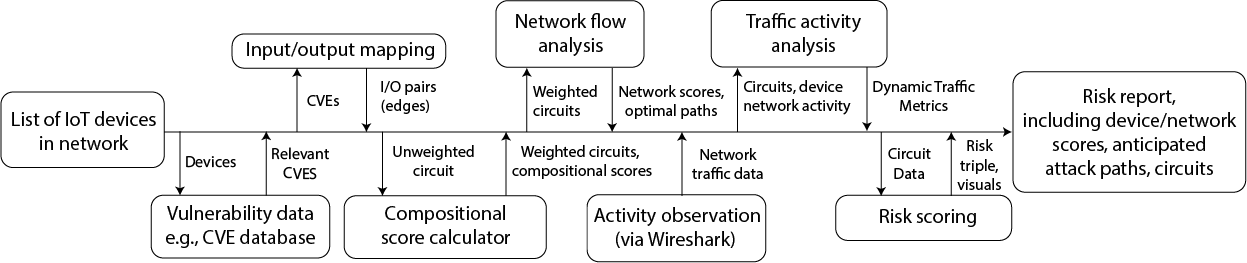
\includegraphics[width=\textwidth]{system_architecture.png}
    \caption{System architecture summary.}
    \label{fig:system_architecture}
\end{figure*}
Our proposal is a sequential computation of the triple $\langle R, E, I\rangle$---a method that utilizes preexisting knowledge about the devices in the network, topology of the network (determined by the relation between different vulnerabilities and potential network flow between devices), and dynamic device activity and network traffic information. This process is outlined in Figure \ref{fig:system_architecture}. At the practical level, the attack circuit model we are proposing considers each of these properties and can provide each of the desired metrics. An attack circuit is a type of flow network \cite{goldberg1989network}, wherein the flows can be used to evaluate level of risk, exploitability, and impact of a network, device, and vulnerability. In this section, we will discuss the nontrivial problem of constructing attack circuits using preexisting knowledge and inferences about IoT devices in the network. We will then explore how the network can then be used to compute \textit{compositional scores} on each of the vulnerabilities, which  provide an important baseline for understanding the initial risk, exploitability, and impact assessments of the network. Then, we'll examine the affect that dynamic network traffic behaviors have on the security of devices in the network and show how these \textit{dynamic metrics} can be combined with the compositional score for a more holistic look at the security of the IoT network. Finally, we'll propose the use of network flow algorithms that make use of the scores we've calculated for anticipating optimal attack paths, which give a final evaluation of the risk, exploitability, and impact measures of the network and its devices. A summary of the implemented system architecture is shown in Figure \ref{fig:system_architecture}.

% To produce a dense representation of possible attacks, the database of vulnerabilities is transformed into flow network graphs . Sources and sinks in the flow network correspond to attack sources and exploited system utilities (attacker targets) respectively. The paths from sources to sinks in the graph are then called \textit{attack circuits}.

\subsection{Circuit Construction}

The attack circuit is constructed in two stages, described in the following sections.

\subsubsection{Input/Output Extraction}
\label{subsubsec:input_output_extraction}

The attack circuits are modeled using text input (vulnerability descriptions) from a vulnerability database. For each item in the database, a corresponding \textit{input/output} pair is generated. The \textit{input} corresponds to the attack source and the \textit{output} corresponds to the attack target. The process is based on TF-IDF \cite{leskovec2014mining} and TextRank \cite{mihalcea2004textrank,PyTextRank} heuristics and is described next as a series of steps.

All text is primed by conversion to lowercase, removal of non-alphanumeric characters, tokenization, stemming \cite{porter1980algorithm,jones1997readings} and subsequent de-tokenization. TF-IDF is then used on the processed corpus to produce an ordering of tokens for each description. TextRank is used on the processed corpus to produce an ordered list of candidate phrases (with Part-Of-Speech (POS) tags) that may best represent the description. The ordered list is filtered to remove noun items (NN). For each item in the list, tokens pruned (limited to a maximum quantity of $3$) based on TF-IDF ordering. Stemming is then removed from tokens by matching them to the corresponding phrase. The result is stored as \textit{input}. This extraction process is then repeated using filtering to remove non-noun items and the result is stored as \textit{output}.

\subsubsection{Graph Composition}

After all of the \textit{input/output} pairs are created, we have the information we need to build the attack circuit structure. In our methodology, an attack circuit is a directed graph isomorphic to a flow network $C = (D,A,S,E)$ where $d \in D$ is a device, represented as a set of vertices that are the set of vulnerability database entries corresponding to $d$; $A$ is the set of attacker vertices; $S$ is the set of target (or sink, as we'll see later) vertices which represent the attack targets in the network; and $E$ is the set of labeled, directed edges. The attack circuit scheme suffices to provide a logical approach to determining which attack targets are at risk. We are more interested, however, in creating variants of the attack circuit that may give insight to the potential impact, exploitability, and overall risk an IoT network yields. To do this, we assign weights and capacities to each of the edges depending on the impact and expoitability scores associated with the respective vulnerability data. A device's impact, exploitability and base scores are then used to compute the attack vector corresponding to its vulnerability. This is used as a component of the device's risk score.

\subsection{Network Composition Analysis}

We're interested in taking a holistic look at devices when evaluating their levels of security and risk. We therefore use several different security metrics that may each be classified into one of two larger categories: compositional scoring and dynamic activity assessment, discussed in the next subsection. Compositional scoring may be performed by observing the device specification, associated vulnerability database information and their corresponding vulnerability scores, and attack circuit topology. Our work incorporates the first two items and designates the third for future work. These compositional scores are derived from the devices themselves and their role in the network composition, and can be calculated irrespective of ways the devices are being used over time. For our work, device's vulnerabilities are scored using the risk base, exploitability, and impact subscore method provided by the existing CVSS v3 standard which accompanies most CVEs. After computing the exploitability and impact subscores for each vulnerability, we can then calculate the compositional score ($c$) of each vulnerability, which is recursively computed using the impact weights and exploitability capacities of the edges of the graph. This is summarized in Equation \ref{eq:exploitability_score} and Equation \ref{eq:impact_score}, where $C_i$ is the set of attack circuit input vertices ($c_i$), where there exists an edge $(c_i,c)$, $C_o$ is the set of attack circuit output vertices ($c_o$), where there exists an edge $(c,c_o)$, and $v_d$ is a dampening constant. The impact and exploitability subscores of each vulnerability of a particular device are then assimilated and transformed (using sigmoidal activation) to determine the impact and exploitability subscores.

\begin{equation}
c_{Exploitability} \mathrel{+}= v_d\sum_{c_i}c_{i_{Exploitability}}
\label{eq:exploitability_score}
\end{equation}

\begin{equation}
c_{Impact} \mathrel{+}= v_d\sum_{c_o}c_{o_{Impact}}
\label{eq:impact_score}
\end{equation}

\subsection{Network Traffic Analysis}

We next examine the dynamic activity metric of a given device in the network. A large body of work is focused on abnormality detection and scoring in network traffic patterns \cite{acar2018peek,apthorpe2017spying,apthorpe2017smart}. A vast variety of metrics may be used for results that shed light onto particular aspects of IoT device and network security. Our work focuses on ascertaining a small number of these metrics from packet sniffing on the network of IoT devices over a period time. The data collected includes device traffic activity, packet content encryption, and the source/destination information of the packets.

To illustrate our use of device traffic activity information, consider the example shown in Figure \ref{fig:usage_over_time}. Devices that are online for the majority of the time (i.e. Google Home Mini, Roku Media Player, HP Printer, and Belkin WeMo) are assigned larger respective multipliers to their exploitability subscore, since their connection leaves them more open to attack by an adversary. The Amazon Echo Dot, in this case, does not have as significant a multiplier applied to its exploitability subscore, since it is not online as frequently.

\begin{figure}[t]
    \centering
    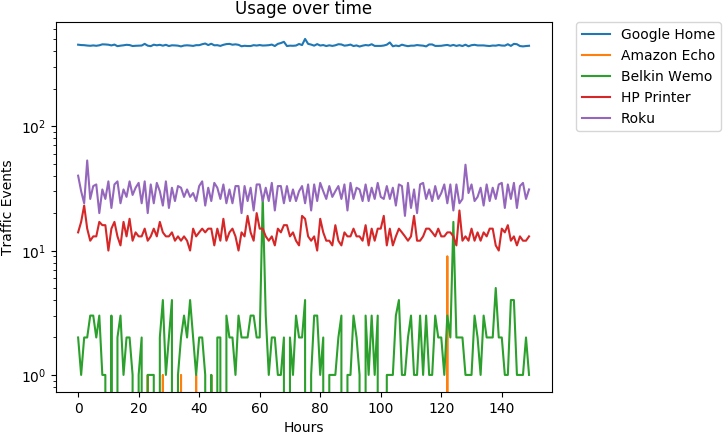
\includegraphics[width=0.5\textwidth]{usageJan14.png}
    \caption{An account of device traffic over a period of $12$ hours.}
    \label{fig:usage_over_time}
\end{figure}

Next, we analyze the percentage of the packets that are sent from and received by each device and their usage of secure encryption protocols. We also check whether any source or destination IP is listed in an IP blacklist database. The encryption metric is used as a multiplier for the exploitability subscore, and the blacklisted IP metric is used as a multiplier for the impact subscore. The calculated the compositional scores and dynamic activity metrics for a device can then be used to improve network analysis and security risk scoring.

\subsection{Network Flows and Attack Path Analysis}

To anticipate how an adversary might carry out an attack on the network and to score the network holistically, we apply a variety of \textit{Network Flow Problems} \cite{Ford-Fulkerson_algo} \cite{dantzig2003max} to the attack circuit for evaluating potential attack paths based on impact, exploitability, and risk. Sources and sinks in the flow network correspond to attack sources and attack targets, respectively.

\subsubsection{Impact Paths} 

An impact path is the route through the circuit that an attacker takes to maximize impact, defined by the circuit edge weights. We specify the attacker nodes as sources, and attacker targets as sinks. Equation \ref{eq:impact_path} illustrates the \textit{Maximum Flow Problem} method used--$f_{uv}$ is the flow between vertices $u$ and $v$, $a$ is an attacker vertex, $s$ is a sink (target) vertex. The sum of the impact path flows of an attack circuit (or the impact score of that circuit) are equivalent to the sum of the total impact of all \textit{easily} accessible attack targets, where the degree of accessibility is defined by the exploitability of the attack paths leading to it.

\begin{equation}
\begin{array}{ll@{}ll}
\text{maximize} & \displaystyle\sum\limits_{} f_{as} & \text{ subject to } \displaystyle\sum\limits_{j} f_{ji} = \displaystyle\sum\limits_{j} f_{ij}
\end{array}
\label{eq:impact_path}
\end{equation}

\subsubsection{Exploitability Paths} 

An exploitability path is a route from attacker to the attack target that is associated with a score  denoting the \textit{resistance} (intuitively, inverse exploitability) of that path. To determine the optimal exploitability paths in a circuit, we solve a \textit{Minimum Cost Flow Problem}, where the cost of an edge is its resistance, or the inverse of the exploitability of that edge (e.g. ($1-$Exploitability), if Exploitability $\in [0,1]$). We use the same sources and sinks as in Equation \ref{eq:impact_path} now with a cost $c_{ij}$ associated with edge $(i,j)$ and a required flow $r_{as}$ from attacker to sink (see Equation \ref{eq:exploitability_path}).

\begin{equation}
\begin{array}{ll@{}ll}
\text{minimize}  & \displaystyle\sum  c_{ij}f_{ij}
\text{ subject to } & \displaystyle\sum f_{as} = r_{as}
\end{array}
\label{eq:exploitability_path}
\end{equation}\\
After computing the optimal exploitability and impact paths, the paths themselves may serve as information for network operators. We may also sum over the exploitability paths in the network to determine an overall network exploitability score, which we then combine with the impact score to improve an overall network security risk score.

\subsubsection{Risk Flow Evaluation} 
Finally, we want to calculate high-risk paths and quantitatively apply these findings to our risk triple. A risk path is a route from attacker to target that is optimized for exploitability constraints, impact weights, and base compositional risk of the vertices. We combine the strategies used in exploitability path and impact path analysis here, solving a \textit{Minimum Cost Maximum Flow Problem} to identify likely paths through the IoT network that an adversary might use in an attack. In Equation \ref{eq:risk_mincost_path}, we outline the network flow problem used to calculate risk, with the usual $c_{ij}$ denoting cost of edge $(i,j)$, $a$ being an attacker vertex (source), and $s$ being a target vertex (sink):
\begin{equation}
\begin{array}{ll@{}ll}
\text{minimize } \displaystyle\sum c_{ij}f_{ij}
\text{ subject to: } \\
\ \ \ \ \text{maximize } \displaystyle\sum\limits_{} f_{as} \text{ subject to } \displaystyle\sum\limits_{j} f_{ji} = \displaystyle\sum\limits_{j} f_{ij}
\end{array}
\label{eq:risk_mincost_path}
\end{equation}
Computing risk paths allow us to calculate an improved risk triple for the network as well as the devices within. The triple $R = \langle R_{Conf}, R_{Integ}, R_{Avail} \rangle$ for a device is calculated using the CVSS v3 metrics for Confidentiality Impact, Integrity Impact, and Availability Impact associated with the CVEs of the device. Flow through each CVE is multiplied by the respective impact metric, and the result defines the risk triple $R$. The numerical values of the impact metrics may be found in table 8.4 of the CVSS v3 specification document\footnote{https://www.first.org/cvss/specification-document}.
% \begin{equation}
%     Base=\begin{cases}
%     0, & \text{Impact subscore $\leq$ 0}\\
%     \min(S_{\text{Impact}} + S_{\text{Exploitability}}, 10), & \text{Scope Unchanged}
    
%   \end{cases}\\
  
% \end{equation}
% \begin{equation}
% Impact=1-[(1-Impact_{\text{Conf}})(1-Impact_{\text{Integ}})(1-Impact_{\text{Avail}})]
% \end{equation}



%%%%%%%%%%%%%%%%%%%%
\section{Implementation}
\label{sec:implementation}

\subsection{Our System}

To understand the performance of our proposed method in common, real-world networks, we model our implementation with off-the-shelf smart home IoT devices. With our implementation based on the NVD, we narrow our focus to the $34$ devices that are both common and have corresponding vulnerabilities listed in the NVD. Live experiments are run on a network consisting of five of these devices: an Amazon Echo Dot, a Belkin WeMo, an HP Inkjet Envy printer, a Google Home Mini, and a Roku digital media player (see Figure \ref{fig:smart_home_network}).

\begin{figure}[t]
    \centering
    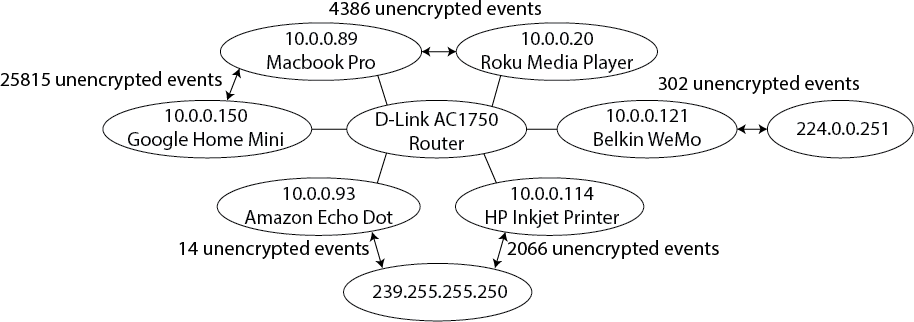
\includegraphics[width=0.5\textwidth]{smart_home_network.png}
    \caption{The smart-home network traffic graph corresponding to Figure \ref{fig:usage_over_time}.}
    \label{fig:smart_home_network}
\end{figure}

Our implementation is based on the CVE vulnerability database. Circuit construction is implemented using relevant CVEs in JSON format from NVD's database, with text processing using the Natural Language Toolkit (NLTK) \cite{bird2004nltk}. An example of the CVE processed as in Section \ref{subsubsec:input_output_extraction} is shown in Figure \ref{fig:processed_cve}. In this example, an \textit{input} (left of the arrow in the i/o field) is an action (DNS rebinding attack) that the attacker needs to take to leverage the corresponding vulnerability, in this case, CVE-2018-11314 (for access to root privileges or the configuration file). For each input, there is an \textit{output} (right of the arrow in the i/o field), which indicates the target that the attacker receives when once the input is applied to the vulnerability. A device may have multiple corresponding CVEs, a CVE may have multiple corresponding inputs, and an input may have multiple corresponding outputs. NetworkX \cite{hagberg2008exploring} and SNAP \cite{leskovec2016snap} are then used to build the attack circuit using these \textit{input/output} pairs and proceed with scoring.

\begin{figure}[t]
    \centering
    \begin{minipage}{0.5\textwidth}
    \begingroup\ttfamily\obeylines
    "Roku Media Player": [\{
    \ "description": "The External Control API in Roku and Roku TV products allow unauthorized access via a DNS Rebind attack.", 
    \ "id": "CVE-2018-11314", 
    \ "i/o": ["DNS Rebinding->this:Root 
    \ Priv", "DNS Rebinding->this:Config 
    \ File"]  \}]
    \endgroup
    \end{minipage}
    \caption{An example of a processed CVE data entry.}
    \label{fig:processed_cve}
\end{figure}

%An example of expoitability and impact attack circuits consisting of three devices (corresponding to the smart-home network shown in Figure \ref{fig:smart_home_network}) are shown in Figure \ref{fig:exploitability_circuit} and Figure \ref{fig:impact_circuit}. The edges of the graph are colored to represent expoitability capacity and impact weight, respectively.
% \begin{figure*}[t]
%     \centering
%     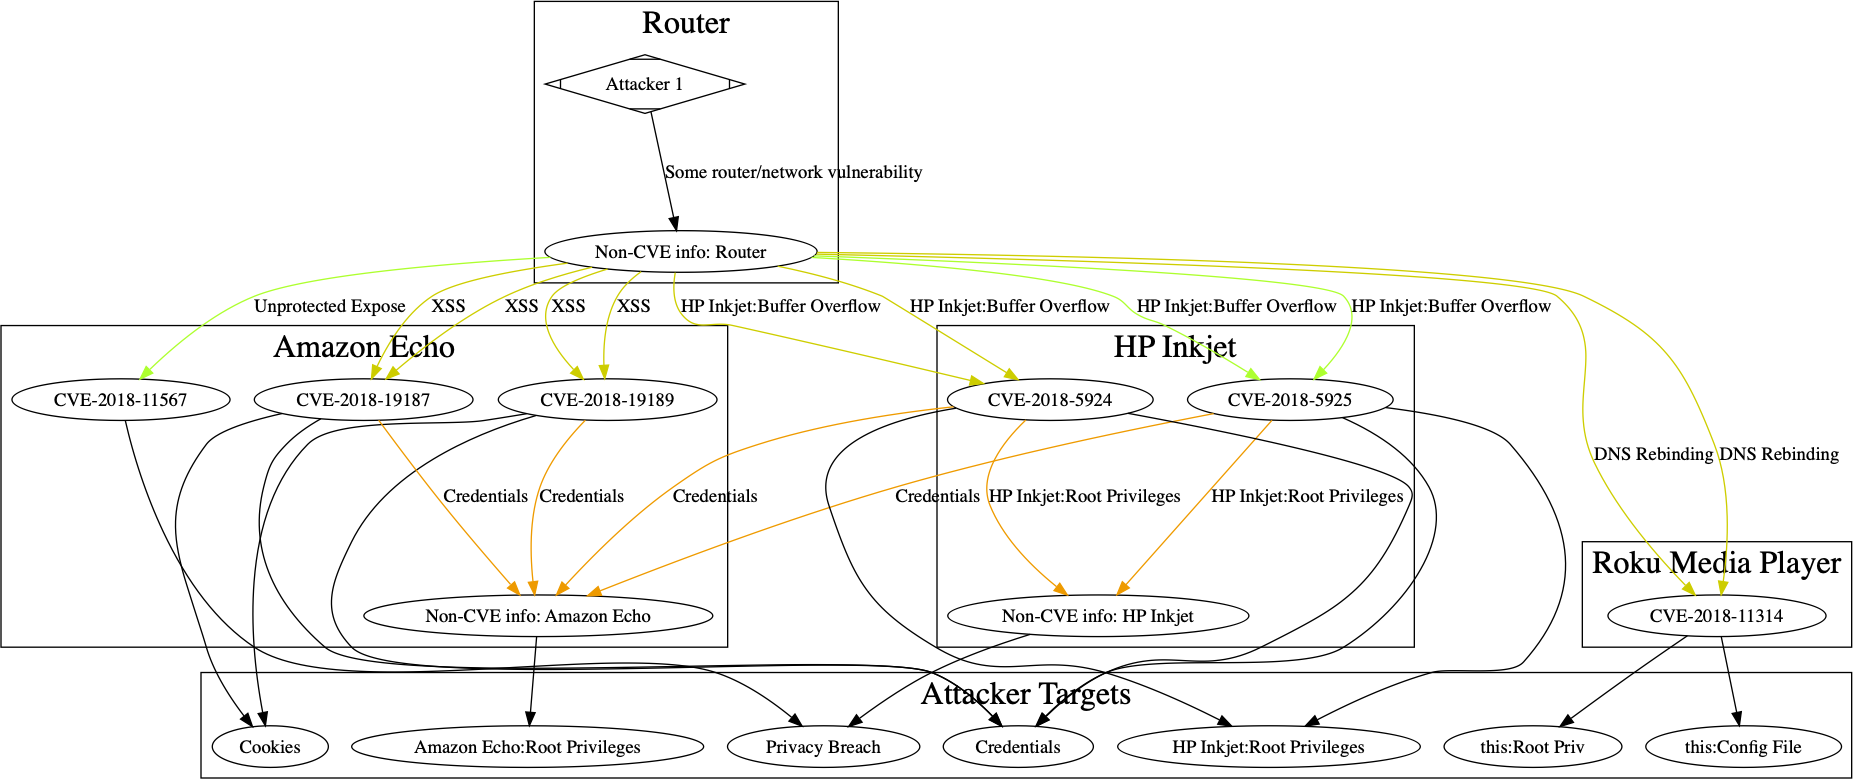
\includegraphics[width=\textwidth]{exploitability_circuit.png}
%     \caption{An example of an exploitability circuit.}
%     \label{fig:exploitability_circuit}
% \end{figure*}

% \begin{figure*}[t]
%     \centering
%     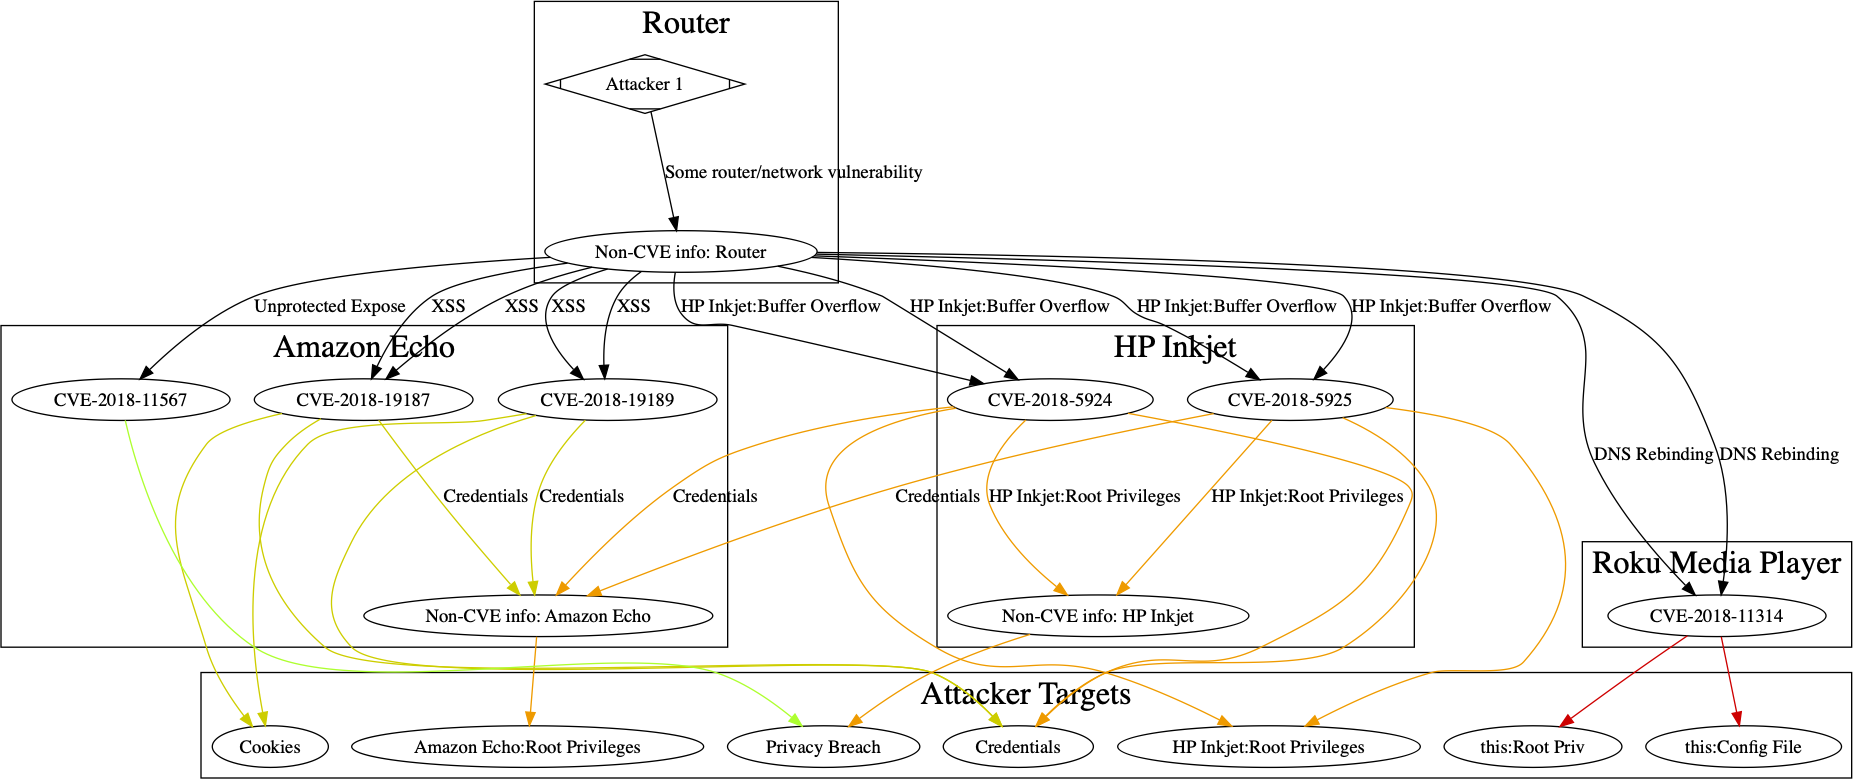
\includegraphics[width=\textwidth]{impact_circuit.png}
%     \caption{An example of an impact circuit.}
%     \label{fig:impact_circuit}
% \end{figure*}
\subsection{Our Scoring Method}

Let $EB_c \in [0,10]$ denote CVE $c$'s base exploitability score and $IB_c \in [0,10]$ denote CVE $c$'s base impact score. $EB_c, IB_c \in [0,10].$ We use impact and exploitability scoring guidelines set by the NVD in their CVSS v3 method\footnote{http://nvd.nist.gov/cvss.cfm}. The numerical possibilities for the CVSS metrics $AV$, $AC$, $PR$, $UI$, $I_{Conf}$, $I_{Integ}$, and $I_{Avail}$ can be found in Table 8.4 of the CVSS specification document. Scoring during the circuit construction phase is computed as shown in Equation \ref{eq:scoring_circuit_construction}. Numerical constants used are assigned based on empirical evaluation of the system. 

\begin{equation}
\begin{array}{ll@{}ll}
EB_c = 8.22 \times AV \times AC \times PR \times UI \\
ISC_{Base} = 1 - [(1-I_{Conf}) \times (1-I_{Integ}) \times (1-I_{Avail})] \\
\texttt{if Scope = unchanged}: IB_c = 6.42 \times ISC_{Base} \\
\texttt{else}: \ \ \  IB_c = 7.52 \times [ISC_{Base}-0.029] \\
\ \ \ \ \ \ \ \ \ \ \ \ \ \ \ \ \ \ \ \ - 3.25 \times [ISC_{Base}-0.02]^{15}
\end{array}
\label{eq:scoring_circuit_construction}
\end{equation}

Then let $EC_d$ denote device $d$'s compositional exploitability score and $IC_d$ denote device $d$'s compositional impact score. Let $c_i$ denote the set of CVEs with input to $c$ (where each device $d$ has a set of $c$ corresponding to each CVE), let $c_o$ denote the set of CVEs that $c$ has output to, and let $v_d$ denote a dampener variable (we used $v_d$ = 0.1). Scoring during the compositional phase is computed as shown in Equation \ref{eq:scoring_compositional}.

\begin{equation}
\begin{array}{ll@{}ll}
EC_d = {\displaystyle\sum_{c \in d}(EB_c+v_d\displaystyle\sum_{i\in c_i}{EB_i}}) \\
IC_d = {\displaystyle\sum_{c \in d}(IB_c+v_d\displaystyle\sum_{o\in c_o}{IB_o}}) \\
\end{array}
\label{eq:scoring_compositional}
\end{equation}

Next we compute the network traffic multipliers for impact and exploitability. Network traffic data is collected using Wireshark \cite{orebaugh2006wireshark} and is stored in .pcap format. This file is then converted to CSV for parsing. The data is specific to a network of $5$ IoT devices and a period of $4$ days. We use three metrics: device Network Uptime ($NU$), Encryption Scheme ($EN$), and whether IP sources or destinations were listed in an IP blacklist database\footnote{https://myip.ms/browse/blacklist} ($IP$). The weights we assigned to the different categories correspond to importance with respect to the score in consideration---for instance, when considering the exploitability score, the Network Uptime multiplier = $NU$ = \texttt{\{"always\_online": 1.6, "frequently\_online": 1.4, "rarely\_online": 1.07, "never\_online": 1\}}.

% \begin{figure}[t]
%     \centering
%     \begin{minipage}{0.5\textwidth}
%     \begingroup\ttfamily\obeylines
%     NU = \{
%     \ "always\_online": 1.6,
%     \ "frequently\_online": 1.4,
%     \ "rarely\_online": 1.07,
%     \ "never\_online": 1
%     \}
%     EN = \{
%     \ "not\_encrypted":1.5, 
%     \ "encrypted": 1
%     \}
%     IP = \{
%     \ "accessed": 5,
%     \ "not\_accessed": 1
%     \}
%     \endgroup
%     \end{minipage}
%     \caption{Category weights.}
%     \label{fig:category_weights}
% \end{figure}

The final exploitability and impact scores $E_d$, $I_d$ for a device $d$ are then calculated as shown in Equation \ref{eq:final_scores}, where $m_{E_i}$ is an exploitability-related network traffic multiplier (e.g. $NU$, $EN$), $m_{I_j}$ is an impact-related network traffic multiplier (e.g. $IP$), and $v_{n}$ is a normalizing variable (we use $v_{n_1}=v_{n_2}=100$). These scores are normalized to a range of $[0,1]$.
\begin{equation}
\begin{array}{ll@{}ll}
E_d = \tanh{(EC_d \times \displaystyle\prod_i m_{E_i} \times v_{n_1})} \\
I_d = \tanh{(IC_d \times \displaystyle\prod_j m_{I_j} \times v_{n_2})} \\
\end{array}
\label{eq:final_scores}
\end{equation}

The overall network exploitability score $E_N$ is defined by the sum of the exploitability scores of its devices, and is accompanied with the path of minimum cost to each of the attack targets. The overall network impact score $I_N$ is the solution to the max-flow problem in the attack circuit after each of the edges have been weighted based on all of the CVEs' base impact scores. Finally, the risk triple $R_N = \langle R_{Conf}, R_{Integ}, R_{Avail} \rangle$ for the network is computed using the CVSS v3 metrics associated with the respective risk triples of the network's devices. First we solve the Maximum Flow Minimum Cost Problem in the attack circuit (see Equation \ref{eq:risk_path_1}). 

\begin{equation}
\begin{array}{ll@{}ll}
\text{minimize } \displaystyle\sum EB_{ij}f_{ij}
\text{ subject to: } \\
\ \ \ \ \text{maximize } \displaystyle\sum\limits_{} IC_{as} \text{ subject to } \displaystyle\sum\limits_{j} f_{ji} = \displaystyle\sum\limits_{j} f_{ij}
\end{array}
\label{eq:risk_path_1}
\end{equation}

Once this is completed, the flow through each CVE is multiplied by the respective impact metric---Confidentiality Impact ($R_C$), Integrity Impact ($R_I$), and Availability Impact ($R_A$), as well as a normalization variable $v_{n_i}$, and the result defines the risk triple $R_d$ for a device $d$ with CVEs $c_i$ (shown in Equation \ref{eq:risk_path_2}). These scores are normalized to range $[0,1]$.

\begin{equation}
\begin{array}{ll@{}ll}
R_{Conf} = \tanh{(v_{n_1}\times R_C\displaystyle\sum_{i} f_{c_i})} \\
R_{Integ} = \tanh{(v_{n_2}\times R_I\displaystyle\sum_{i} f_{c_i})} \\
R_{Avail} = \tanh{(v_{n_3}\times R_A\displaystyle\sum_{i} f_{c_i})} \\
\end{array}
\label{eq:risk_path_2}
\end{equation}
\section{Evaluation}
\label{sec:evaluation}

\begin{figure}[t]
    \centering
    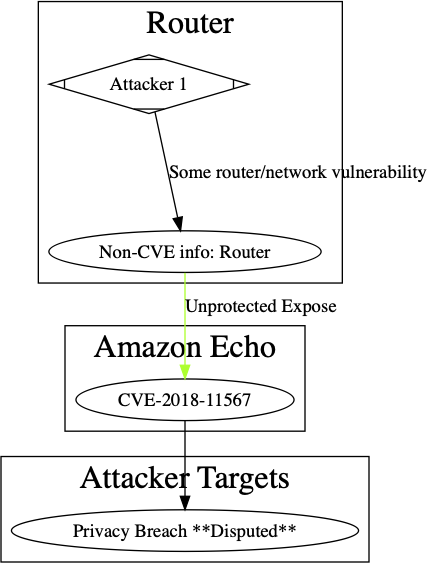
\includegraphics[width=0.20\textwidth]{exploitability_circuit1cve.png}
    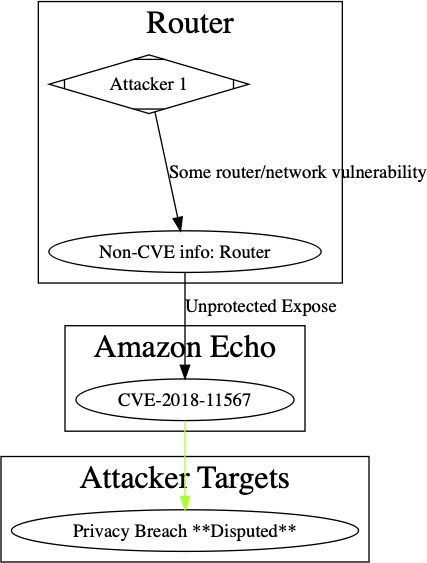
\includegraphics[width=0.20\textwidth]{impact_circuit1cve.png}
    \caption{Exploitability (left) and impact (right) circuits corresponding to one device under the observation of a single vulnerability.}
    \label{fig:exp1cve}
\end{figure}

\begin{figure}[t]
    \centering
    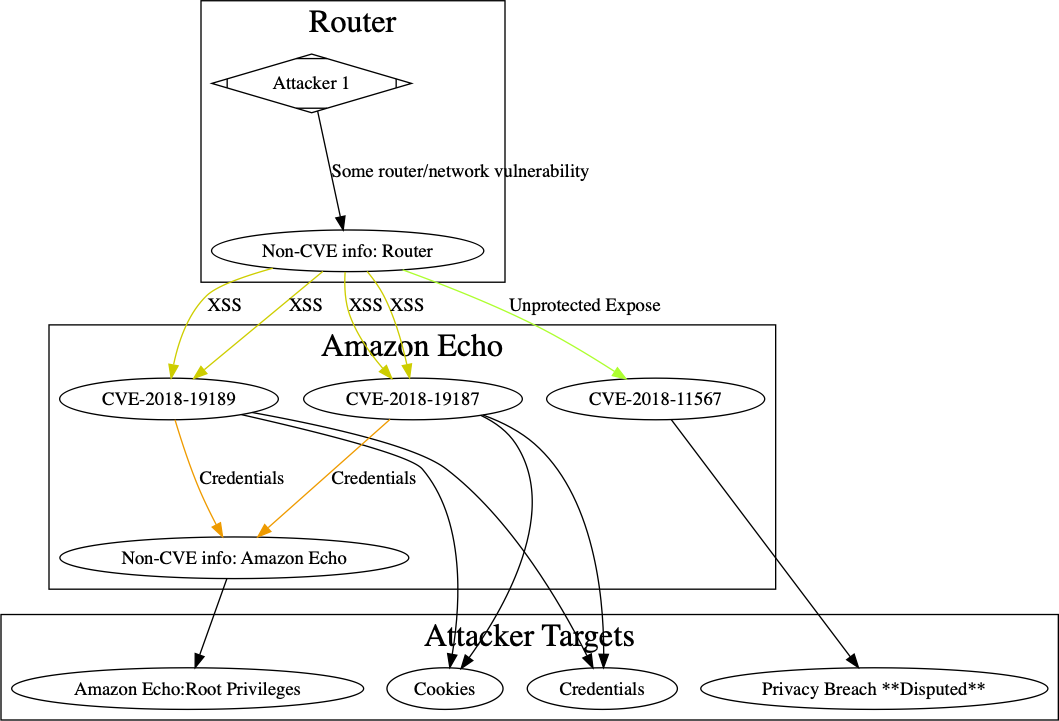
\includegraphics[width=0.40\textwidth]{exploitability_circuit1dev.png}
    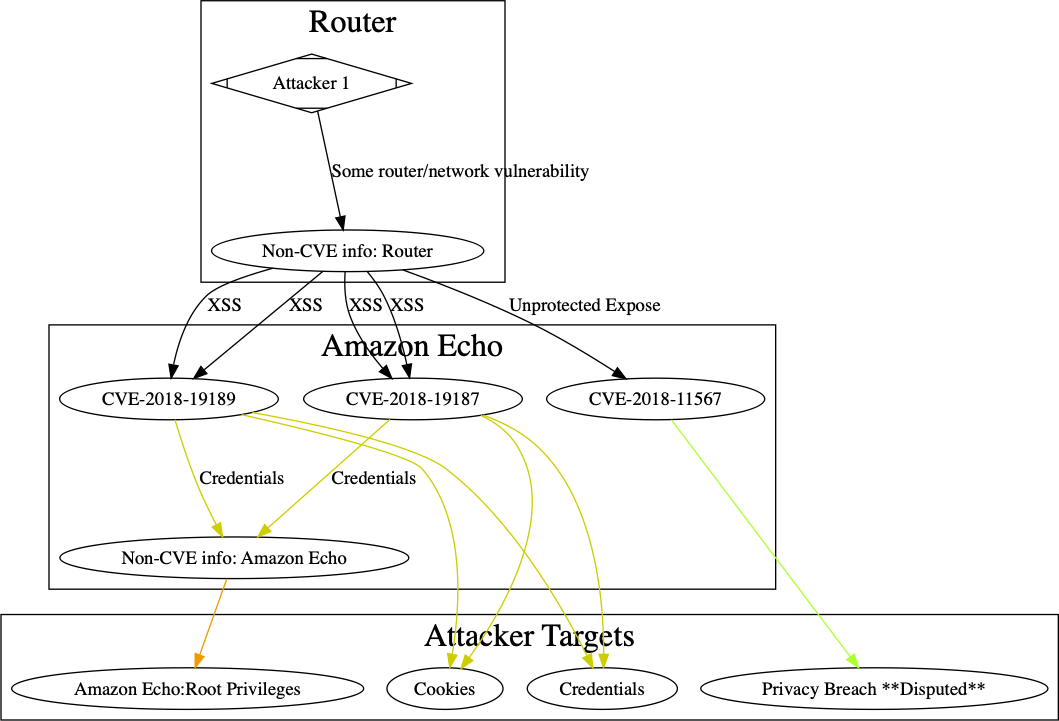
\includegraphics[width=0.40\textwidth]{impact_circuit1dev.png}
    \caption{Exploitability (top) and impact (bottom) circuits corresponding to one device under the observation of all vulnerabilities.}
    \label{fig:exp1dev}
\end{figure}

\begin{figure*}[t]
    \centering
    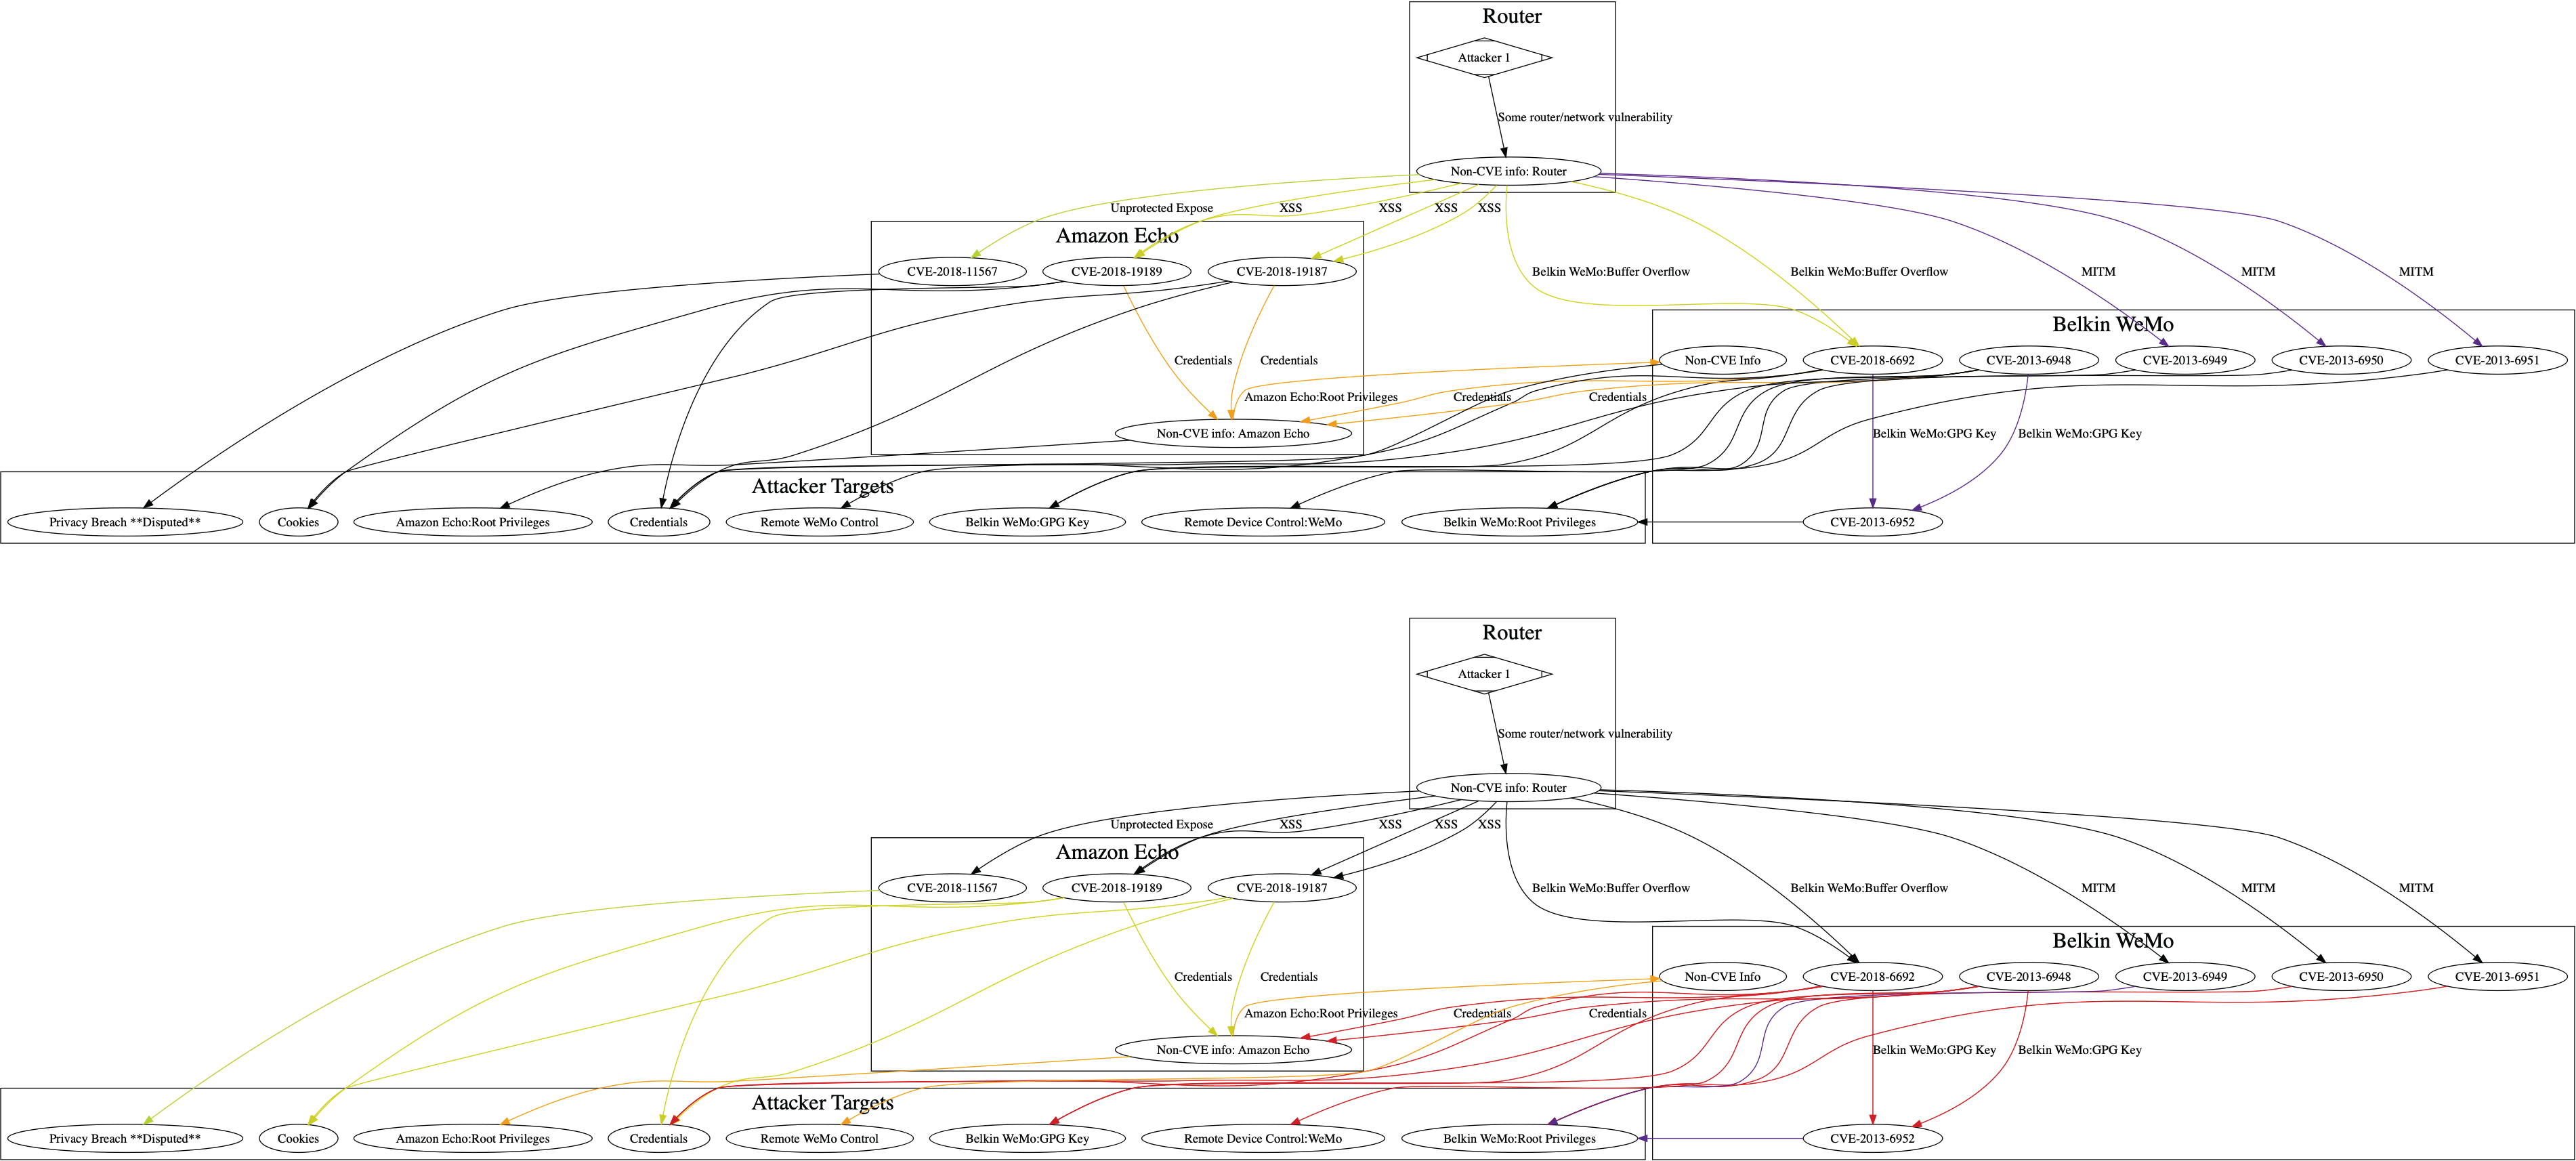
\includegraphics[width=\textwidth]{both2devallcve.png}
    \caption{Exploitability (top) and impact (bottom) circuits corresponding to two devices under the observation of all vulnerabilities. Full-sized images are available in the repository.}
    \label{fig:exp2dev}
\end{figure*}

We evaluate the attack circuit system using a variety of networks and device activity metrics. In our work, we showcase three of these networks: one consisting of one device (an Amazon Echo Dot) with one vulnerability (CVE-2018-11567), one consisting of the Amazon Echo Dot and all of its corresponding CVEs, and one consisting of the Amazon Echo Dot, a Belkin WeMo smart plug, and all of their associated CVEs. The generated exploitability and impact circuits for each of the three settings are shown at the back of this paper in Figures \ref{fig:exp1cve}, \ref{fig:exp1dev}, and \ref{fig:exp2dev}, respectively. Note that the attack circuit complexity grows exponentially with respect to the number of devices in the network, which is visually evident in these figures and is the reason why we primarily focus on smaller networks to demonstrate our work. 

In Table \ref{tab:results}, we record the scores of devices and the network as they were calculated with each of the networks. These results reflect the dynamic activity metrics that we recorded in our experimental observation of the devices over a period of $4$ days, and the output values respond accordingly as we experimentally change the dynamic metrics of the devices (for instance, in contrast to the 1-CVE, 1-device network yielding an exploitability score of $0.0289$ with the Echo's actual status of ``\texttt{rarely\_online}", we noted that the exploitability score rose to $0.0378$ when the device was marked as ``\texttt{frequently\_online}"). Note that where only one device is used, the Belkin WeMo scores are N/A because the device is not present in that network. We select these particular devices to evaluate and illustrate the change in scores when two devices of different levels of vulnerability are added to a network. Based on its three total CVEs, the Amazon Echo's vulnerabilities don't yield as high of a risk, exploitability, or impact score of the device. Its CVEs CVE-2018-11567, CVE-2018-19189, and CVE-2018-19187 have base exploitability scores of $1.8$, $2.8$, and $2.8$, and base impact scores of $1.4$, $2.7$, and $2.7$, respectively. In contrast, three of the Belkin WeMo's six CVEs (CVE-2018-6692, CVE-2013-6952, and CVE-2013-6949) are serious vulnerabilities with base exploitability scores of $3.9$, $10.0$, and $8.6$, and base impact scores of $6.0$, $10.0$, and $10.0$, respectively. Note that in the first column, we observe a network with a vulnerability that is of relatively lesser concern (CVE-2018-11567, with a base exploitability score of $1.8$ and base impact score of $1.4$). When more vulnerabilities are added in, the device's scores all increase as expected, and the network score increases in the same way (because in this setting, the network is defined solely by the device). When the WeMo is added, several paths between the WeMo's vulnerabilities and the Echo's vulnerabilities are discovered from the I/O mapping step, which causes each of the Echo's scores to rise, and the network's scores likewise undergo an increase with the introduction of these new vulnerabilities.

\begin{table}[t]
    \centering
    \begin{tabular}{| c | c | c | c |}
    \toprule
    {} & Echo, 1 CVE & Echo, all CVEs & Echo, WeMo \\
    \midrule
    $E_{Echo}$ & 0.0289 & 0.1182 & 0.3380 \\
    $I_{Echo}$ & 0.0140 & 0.0679 & 0.1776 \\
    Echo $R_{Conf}$ & 0.0073 & 0.0341 & 0.0982 \\
    Echo $R_{Integ}$ & 0.0 & 0.0268 & 0.0910 \\
    Echo $R_{Avail}$ & 0.0 & 0.0 & 0.0644 \\
    \midrule
    $E_{WeMo}$ & N/A & N/A & 0.8490 \\
    $I_{WeMo}$ & N/A & N/A & 0.4823 \\
    WeMo $R_{Conf}$ & N/A & N/A & 0.5744 \\
    WeMo $R_{Integ}$ & N/A & N/A & 0.5649 \\
    WeMo $R_{Avail}$ & N/A & N/A & 0.4605 \\
    \midrule
    $E_{Network}$ & 0.0289 & 0.1182 & 0.9223 \\
    $I_{Network}$ & 0.0140 & 0.0679 & 0.6078 \\
    Network $R_{Conf}$ & 0.0073 & 0.0341 & 0.6367 \\
    Network $R_{Integ}$ & 0.0 & 0.0268 & 0.6239 \\
    Network $R_{Avail}$ & 0.0 & 0.0 & 0.5098 \\
    \bottomrule
    \end{tabular}
    \\
    \caption{Device and network scores for different network settings.}
    \label{tab:results}
\end{table}

\begin{figure}[t]
    \centering
    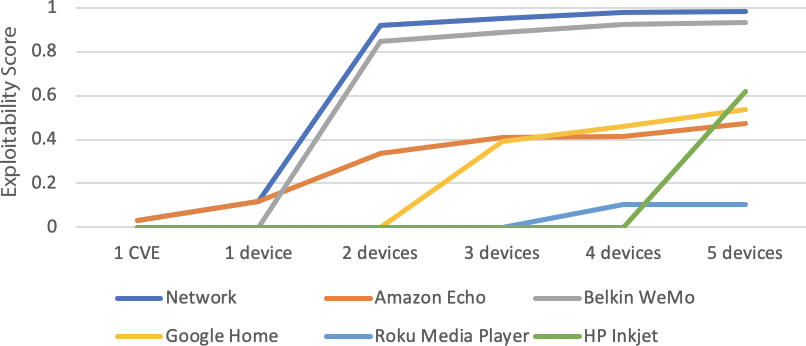
\includegraphics[width=0.45\textwidth]{exploitability_trends.png}
    \caption{Exploitability score adjustment with the addition of new devices (augmented in sequence (left to right, top to bottom)) and CVEs.}
    \label{fig:exploitability_trends}
\end{figure}

This then raises the following question: how can the scores of networks, which are largely heterogeneous and unique, be interpreted relativistically? This is a difficult problem to address, especially without data from real attack circuit use. For now, we normalize the score to a range of $[0,1]$ using a sigmoidal ($\tanh$) function. In general, as the number of devices grows and the vulnerabilities increase, the score trends will demonstrate a sigmoidal behavior, converging to $1$. In Figure \ref{fig:exploitability_trends}, we observe one metric---the exploitability score---of $5$ devices and the overall network, and how it changes as more devices are added. In particular, we start with the Amazon Echo with one vulnerability, then add the rest of the Amazon Echo's vulnerabilities, then add the Belkin WeMo, the Google Home Mini, the Roku media player, and finally the HP Inkjet printer in sequence. As expected, the network's exploitability score approaches a value of $1$ as more devices are added. The case may be made that this scoring method is too sensitive (regardless of the fact that these networks are comprised of devices whose vulnerabilities we know). This may be a result of the dampener and normalization variable values or lack of information about attack circuit behavior in practice. We leave the related refinement of the scoring method to future work.

% Experimental results:

% 1 device (amazon echo), 1 CVE (CVE-2018-19189)
% Echo exploitability:  0.0481128237946 Echo impact:  0.0299910032388 (Echo exploitability:  0.0629167831126 if frequently online)
% Network exploitability:  0.0481128237946 Network impact:  0.0299910032388

% \begin{table}[t]
%     \centering
%     \begin{tabular}{| c | c | c |}
%     \toprule
%     {} & Exploitability Score & Impact Score \\
%     \midrule
%     Echo & 0.0481 & 0.0299 \\
%     Network & 0.0481 & 0.0299 \\
%     \bottomrule
%     \end{tabular}
%     \caption{Device and network exploitability for a network consisting of one device (Amazon Echo) and one CVE item (CVE-2018-19189). Note that if the device is frequently online, the exploitability score changes to $0.0629$.}
%     \label{tab:1cve}
% \end{table}

% 1 device (amazon echo), all CVEs
% Echo exploitability:  0.168507357322 Echo impact:  0.105604770889 (Echo exploitability:  0.21899477347 if frequently online)
% Network exploitability:  0.168507357322 Network impact:  0.105604770889

% Echo exploitability:  0.0288819651753 Echo impact:  0.013999085405 Echo risk confidentiality:  0.0072598724503 Echo risk integrity:  0.0 Echo risk avalilability:  0.0
% Network exploitability:  0.0288819651753 Network impact:  0.013999085405 Network risk confidentiality:  0.0072598724503 Network risk integrity:  0.0 Network risk avalilability:  0.0
% Echo exploitability:  0.118214664357 Echo impact:  0.067895382829 Echo risk confidentiality:  0.0340867888711 Echo risk integrity:  0.0268335568068 Echo risk avalilability:  0.0
% Network exploitability:  0.118214664357 Network impact:  0.067895382829 Network risk confidentiality:  0.0340867888711 Network risk integrity:  0.0268335568068 Network risk avalilability:  0.0
% Echo exploitability:  0.33798508168 Echo impact:  0.177596681443 Echo risk confidentiality:  0.0982420955039 Echo risk integrity:  0.091047160172 Echo risk avalilability:  0.0643708690678
% WeMo exploitability:  0.848966437613 WeMo impact:  0.482286842811 WeMo risk confidentiality:  0.574356582125 WeMo risk integrity:  0.564899552846 WeMo risk avalilability:  0.460542808826
% Network exploitability:  0.922306690621 Network impact:  0.607822022468 Network risk confidentiality:  0.636673729467 Network risk integrity:  0.623860031885 Network risk availability:  0.509800370196

% \begin{table}[t]
%     \centering
%     \begin{tabular}{| c | c | c |}
%     \toprule
%     {} & Exploitability Score & Impact Score \\
%     \midrule
%     Echo & 0.1685 & 0.1056 \\
%     Network & 0.1685 & 0.1056 \\
%     \bottomrule
%     \end{tabular}
%     \caption{Device and network exploitability for a network consisting of one device (Amazon Echo) and all CVE items. Note that if the device is frequently online, the exploitability score changes to $0.2189$.}
%     \label{tab:1dev}
% \end{table}



% 2 devices
% Echo exploitability:  0.187157640205 Echo impact:  0.117455355915
% WeMo exploitability:  0.610551402738 WeMo impact:  0.325690709881
% Network exploitability:  0.715903238257 Network impact:  0.426818500412

% \begin{table}[t]
%     \centering
%     \begin{tabular}{| c | c | c |}
%     \toprule
%     {} & Exploitability Score & Impact Score \\
%     \midrule
%     Echo & 0.1871 & 0.1174 \\
%     WeMo & 0.6105 & 0.3256 \\
%     Network & 0.7159 & 0.4268 \\
%     \bottomrule
%     \end{tabular}
%     \caption{Device and network exploitability for a network consisting of two devices (Amazon Echo, Belkin WeMo) and all CVE items.}
%     \label{tab:2dev}
% \end{table}
\section{Conclusion}
\label{sec:conclusion}

In this paper, we address the problem of evaluating the security of a network. This is done by using \textit{attack circuits} and associated compositional scores and dynamic activity metrics. In this manner, an individual IoT device or network may be analyzed for its vulnerability to security attacks. Evaluation in Section \ref{sec:evaluation} demonstrates the increased security risks for a growing IoT network. While our work focuses on using descriptions to extract \textit{input/output} pairs, this approach may be extended to extract multiple pairs per description, as well as using other available information sources. Activity metrics may be further developed by using generative machine learning models to learn abnormal network traffic behaviors. We also noted that as networks grow, their complexity grows exponentially. Thus, the network flow problems described may become inefficient with huge IoT attack circuits, and alternative approaches like graph neural networks (GNNs) \cite{Scarselli09thegraph} may be required for their analysis. However, for application in smaller IoT networks (e.g. smart homes), we conclude that this approach suffices.

%we use 3 metrics (for now)

% adding network-particular score relativizing as future work



%the bib
%\footnotesize
\bibliographystyle{IEEEtran}
\bibliography{IEEEabrv,references}
%\input{appendix.tex}
\end{document}
